\chapter{Konzeption} \label{chapter:conception}

In diesem Abschnitt wurden, auf Basis der formalen Anforderungen,
Funktionalitäten des Frameworks konzipiert. Hierbei wurde auf den
Funktionalitäten des bestehenden Systems aufgebaut und weitere Funktionalitäten
hinzugefügt, um die Anforderungen abzudecken. Anschließend wurde das
Interface-Design der Frame\-work-Kom\-po\-nen\-ten entwickelt. Abschließend wurde
auf Grundlage der Anforderungen die zu nutzenden Frameworks festgelegt und
darauf aufbauend die Systemarchitektur festgelegt.

\section{Funktionalität} \label{sec:concept-func}

Im Folgenden werden die konzipierten Funktionalitäten des Systems
vorgestellt, welche die zuvor festgelegten Anforderungen (vgl.
\autoref{sec:analysis-anf}) erfüllen sollen. Zuerst werden die übernommenen und
überarbeiteten Funktionalitäten der EMI-Award-App dargelegt. Anschließend werden
neue Funktionalitäten vorgestellt.

\subsection{Übernommene und angepasste Funktionalitäten}

Die Funktionalitäten der EMI-Award-App (vgl. \autoref{table:emi-func}) dienen für
diese Arbeit als Grundlage. Um die Systemarchitektur später einfacher abbilden
zu können, werden die Funktionalitäten nach Nutzungsgruppe gruppiert (vgl.
\autoref{table:funk-old}). Aufgrund der abweichenden Anforderungen zur
EMI-Award-App müssen einige Funktionalitäten angepasst werden. Im Folgenden
werden die übernommenen und überarbeiteten Funktionalitäten für Veranstaltende
und Teilnehmende präsentiert.

\begin{table}[htpb]
    \def\arraystretch{1.25}
    \centering
    \caption{Übernommene Funktionalitäten der EMI-Award-App für (T)eilnehmende und (V)eranstaltende}
    \label{table:funk-old}
    \begin{tabular}{lll}
        \uzlhline%
        \uzlemph{ID} & \uzlemph{Titel}                            & \uzlemph{Anforderungen} \\
        \uzlhline%
        Ft-V-1       & Eintragen und Verwalten von Stationen      & \anfref{F11}            \\
        Ft-V-2       & Eintragen und Verwalten von Abzeichen      & \anfref{F12}            \\
        Ft-V-3       & Eintragen und Verwalten von Hilfseinträgen & \anfref{F13}            \\
        Ft-V-4       & Eintragen und Verwalten der Einführung     & \anfref{F14}            \\
        Ft-T-1       & Interaktive Karte mit Stationen            & \anfref{F30}            \\
        Ft-T-2       & Auflistung der Stationen                   & \anfref{F30}            \\
        Ft-T-3       & Virtuelles Besuchen mit QR-Code            &                         \\
        Ft-T-4       & Abzeichen                                  & \anfref{F60}            \\
        Ft-T-5       & Bedienungshilfe                            & \anfref{F50}            \\
        Ft-T-6       & Einleitende Slideshow                      & \anfref{F40}            \\
        \uzlhline
    \end{tabular}
\end{table}

Für die Veranstaltenden wurden einige Anpassungen vorgenommen. Das Eintragen der
Stationen (Ft-V-1), Abzeichen (Ft-V-2), Hilfseinträge (Ft-V-3) und Einführung
(Ft-V-4) muss an die Verallgemeinerung des Frameworks angepasst werden. Da der
Kontext der EMI-Award-App sehr spezifisch ist, waren die Anpassungsmöglichkeiten
auf das nötige beschränkt. Konkret wurden einige Daten in der App fest
eingebaut. Dies umschließt die Icons von Stationen und Abzeichen, die
Abschlussbedingung der einzelnen Abzeichen, sowie die Bilder der Einführung. All
diese Einstellungen sollten frei anpassbar sein. Zudem werden mediale Inhalte
für Stationen nun nicht mehr benötigt, da diese nicht für jede Veranstaltung von
Bedeutung sind. Icons hingegen müssen für Stationen angegeben werden.
\\
Zusätzlich werden zwei neue Abschlussbedingungen eingeführt: eine
Textabgabe und eine Bildabgabe, welche von Veranstaltenden manuell akzeptiert
oder abgelehnt werden können.

Die Hilfseinträge (Ft-V-3) werden weitergehend überarbeitet, um eine größere
Anzahl an Einträgen übersichtlich anzuzeigen. Hierzu werden die Einträge
nach Kategorie gruppiert und in einem \ac{FAQ} Format angegeben.
Somit wäre eine mögliche Frage „Wann endet die Veranstaltung?“, eingeordnet in
der Kategorie „Organisatorisches“.

Eine weitere Überarbeitung betrifft das Eintragen und Verwalten der Einführung
(Ft-V-4), welche nun weitere Folienformate unterstützt. Das Layout der
EMI-Award-App hat ein festgesetztes Bild mit anpassbarem Text darunter
angezeigt. Stattdessen werden drei neue Formate eingeführt: Titelfolie (Bild +
Text), Bildfolie (Text + Bild) und eine ausschließliche Textfolie.

\subsection{Neue Funktionalitäten} \label{ssec:func-new}

Um alle aufgestellten Anforderungen abzudecken, wurden zudem einige neue
Funktionalitäten konzipiert. Diese werden in \autoref{table:funk-new}
präsentiert und im Folgenden näher ausgeführt.

\begin{table}[htpb]
    \def\arraystretch{1.25}
    \centering
    \caption{Neue Funktionalitäten}
    \label{table:funk-new}
    \begin{tabular}{lll}
        \uzlhline%
        \uzlemph{ID} & \uzlemph{Titel}                    & \uzlemph{Anforderungen}   \\
        \uzlhline%
        Ft-V-5       & Benachrichtigungen an Teilnehmende & \anfref{F70}              \\
        Ft-V-6       & Feedbackanfragen                   & \anfref{F80}              \\
        Ft-V-7       & Statistiken zur Veranstaltung      & \anfref{F20}              \\
        Ft-V-8       & Zentrales Dashboard zur Verwaltung & \anfref{F10}~\anfref{F90} \\
        Ft-T-7       & Gruppen                            & \anfref{F100}             \\
        Ft-T-8       & Manuelle Abzeichen                 & \anfref{F60}              \\
        \uzlhline
    \end{tabular}
\end{table}


Die Benachrichtigungen (\textit{Ft-V-5}) können von Veranstaltenden über das
Dashboard (\textit{Ft-V-8}) an Teilnehmende gesendet werden. Die
Benachrichtigungen bestehen dabei aus Titel und einem Textinhalt. Alle bereits
gesendeten Benachrichtigungen können in einer Tabelle eingesehen werden. Die
Teilnehmenden erhalten beim Senden einer Benachrichtigung in der Web-App eine
Push-Benachrichtigung, welche die Eingaben der Veranstaltenden beinhaltet.
Sollten Teilnehmende zum Zeitpunkt des Absendens der Benachrichtigung die
Web-App nicht offen haben, so wird die Benachrichtigung zum nächsten Öffnen der
App präsentiert.

Die Feedbackanfragen (\textit{Ft-V-6}) geschehen in ähnlicher Form wie
\textit{Ft-V-5}. Erneut können Veranstaltende über das Dashboard
(\textit{Ft-V-8}) Anfragen abschicken, welche Teilnehmende mit einem
Feedbackdialog präsentiert. Im Gegensatz zur Benachrichtigung können
Veranstaltende bei einer Feedbackanfrage einen Titel und auswählbare Gründe für
ein schlechtes Feedback angeben, um jedem Veranstaltungstypen gerecht zu werden.
Teilnehmende können aus drei möglichen Bewertungen wählen: „Gut“, „Mittelmäßig“
und „Schlecht“, welche als Emojis präsentiert werden. Bei einer Wahl von
„Mittelmäßig“ oder „Schlecht“ können Teilnehmende anschließend aus den, von
Veranstaltenden vorgegebenen, Gründen auswählen und alternativ einen eigenen
Grund angeben. Das abgesendete Feedback wird Veranstaltenden anschließend im
Dashboard präsentiert.

Zusätzlich werden auch die Statistiken (\textit{Ft-V-7}) im Dashboard
(\textit{Ft-V-8}) angezeigt. Diese werden unterteilt in „Stationen“,
„Abzeichen“, „Teilnehmende“ und „Feedback“. Zu Stationen, Abzeichen und
Teilnehmenden werden die kumulativen, täglichen und durchschnittlichen Besuche
pro Tag, neue Teilnehmende und Abzeichenabschlüsse angezeigt. Für Stationen und
Abzeichen werden zusätzlich die kumulativen Besuche und Abschlüsse pro Station
und Abzeichen angezeigt. Die kumulativen und täglichen Daten werden in Form
eines Graphen angezeigt. \\
In der Kategorie Feedback werden die insgesamt eingetroffenen Antworten, ihre
Bewertungen und die drei häufigsten angegebenen Gründe für schlechte Bewertungen
angezeigt. Zudem werden alle Antworten individuell in einer Tabelle dargestellt,
in der auch die eigenen Gründe der Teilnehmenden vorhanden sind.

Das Dashboard (\textit{Ft-V-8}) beinhaltet, neben den bereits erläuterten
Funktionen, eine Ansicht zur Bearbeitung der eingereichten Text- und
Bildabzeichen, sowie Eintragung und Verwaltung der Rahmendaten. Alle offenen
Einreichungen für Abzeichen, welche einer manuellen Bearbeitung bedürfen, werden
in einer Liste angezeigt und können ausgewählt werden, um die Einreichung zu
betrachten und zu bewerten. Die Rahmendaten der Veranstaltung lassen sich
separat davon verwalten. Sie umfassen Titel, Logo, Anfang und Ende der
Veranstaltung, sowie optionale Funktionen, einen Link zu weiteren Informationen
der Veranstaltung, das initiale Zentrum der interaktiven Karte und rechtliche
Informationen wie Impressum und Datenschutzerklärung.

Des Weiteren haben Teilnehmende die Möglichkeit Aktivitäten als Gruppen
(\textit{Ft-T-7}) abzuschließen. Hierzu gehört das Besuchen von Stationen und
das Abschließen von Abzeichen. Beim ersten Aufruf wird Teilnehmenden die
Möglichkeit gegeben, eine Gruppe zu erstellen oder einer Gruppe beizutreten.
Dies geschieht über das Scannen des QR-Codes eines Gruppenmitglieds oder
alternativ mit der manuellen Eingabe des Gruppen-Codes. Zudem können
Teilnehmende die Gruppe jederzeit verlassen, eine neue erstellen oder einer
anderen beitreten. Die Gruppen-Funktion kann von Veranstaltenden im Dashboard
(\textit{Ft-V-8}) eingestellt werden. Gruppen können erforderlich, optional oder
ausgeschaltet sein.

Abschließend stellen manuelle Abzeichen (\textit{Ft-T-8}) die letzte neue
Funktionalität dar, welche die manuelle Bearbeitung durch Veranstaltende
benötigen. Dazu gehören Text- und Bildabzeichen, sowie das manuelle Bestätigen
eines Abzeichens. Durch sie erhalten Teilnehmende die Möglichkeit kleine Texte
oder Bilder bei entsprechenden Abzeichen abzugeben. Nach der Abgabe können
Veranstaltende, wie in der Dashboard-Funktionalität beschrieben, die Einreichung
akzeptieren oder ablehnen. Sollte die Einreichung abgelehnt werden, können
Teilnehmende erneut eine Abgabe einreichen. Andernfalls wird das Abzeichen als
abgeschlossen markiert. \\
Insgesamt gibt es somit nun folgende Abschlussbedingungen: \textit{Anzahl
    besuchter Stationen}, \textit{Abschließen aller (anderen) Abzeichen},
\textit{Textabgabe}, \textit{Bildabgabe} und \textit{Manuelles akzeptieren}.

\section{Frameworks} \label{sec:frameworks}

Da die Wahl von Frameworks aufgrund der unterschiedlich Arbeitsweisen und
Funktionalitäten einen großen Einfluss auf das Interface-Design und die
Systemarchitektur hat, werden an dieser Stelle die im Rahmen der vorliegenden
Arbeit eingesetzten Frameworks vorgestellt und begründet festgelegt. Die
Grundlage der Auswahl bilden die genutzten Frameworks der EMI-Award-App, welche
bereits in \ssecref{ssec:analysis-old-tech} aufgeführt wurden. Dabei wird
überprüft, ob die genutzten Frameworks die neuen Anforderungen aus
\autoref{sec:analysis-anf} berücksichtigen.

Nach wie vor werden Web-Frameworks vorausgesetzt (\anfref{R10}). Auf der Seite
des Teilnehmenden sollten diese zur offline Verfügbarkeit (\anfref{Q60}) die
Nutzung von \acp{PWA} unterstützen. Da \acp{PWA} eine gesicherte Verbindung
benötigen, ist die Unterstützung von HTTPS (\anfref{Q70}) ebenfalls nötig. Zudem
muss die Darstellung von \ac{AR}/\ac{VR}-Inhalten (Ft-T3) möglich sein.
Zusätzlich sollten die Frameworks ausgereift und umfassend getestet
(\anfref{R60}, \anfref{Q30}), sowie performant und kompakt sein (\anfref{R30},
\anfref{Q80}). Auf Seite der Veranstaltenden sollte das Framework das
übersichtliche Verwalten der eingetragenen Informationen ermöglichen
(\anfref{F10}) und um die vorgesehenen Funktionen aus \autoref{sec:concept-func}
erweiterbar sein.

\urldef\strapidep\url{https://github.com/strapi/strapi/network/dependents?package%5Fid=UGFja2FnZS0xODMyNjEwNQ%3D%3D}

Unter Beachtung dieser Anforderungen werden die Frameworks der EMI-Award-App nun
erneut betrachtet. Die Grundlage des Frontends bildet der progressive JavaScript
Framework \textit{Vue.js}. Bei der Nutzung von Vue CLI kann die
PWA-Funktionalität mithilfe des \textit{@vue/cli-plugin-pwa} Pakets schnell
eingebunden werden. Zudem ist Vue.js mit 33.6kB \cite[{v3.2.29, minifiziert und
            komprimiert}]{Kanodia2022} ein kompaktes Framework und kleiner als die zwei
größten Konkurrenten Angular (62.3kB) und React (42.2kB). Ebenfalls schneidet
Vue.js in Leistungs-Benchmarks besser ab \cite{Krause2022}. Weiterhin ist Vue.js
mit 192.814 GitHub-Sternen\footnote{Stand 05.02.2022,
    https://github.com/vuejs/vue} das beliebteste Framework (React
181.881\footnote{Stand 05.02.2022, \url{https://github.com/facebook/react}},
Angular 79.393\footnote{Stand 05.02.2022,
    \url{https://github.com/angular/angular}}). \\
Für die Einbindung der \ac{AR}/\ac{VR}-Inhalte wurde in der EMI-Award-App
\textit{A-Frame} genutzt. Bei A-Frame handelt es sich einen um Web-Framework für
\ac{XR} Erlebnisse, welcher auf der bekannten\footnote{Stand 06.02.2022: 78.787
GitHub-Sterne} JavaScript Bibliothek
\textit{Three.js}\footnote{\url{https://github.com/mrdoob/three.js}} aufbaut.
Mit 13.696 GitHub-Sternen\footnote{Stand 06.02.2022,
\url{https://github.com/aframevr/aframe/}} ist A-Frame eines der beliebtesten
Frameworks für \ac{VR}/\ac{AR}-Inhalte im Web-Kontext. Die
Vorzeigeprojekte\footnote{\url{https://aframe.io/showcase/}} des Frameworks und
Anzahl der GitHub-Sterne weisen hier ebenfalls auf seinen ausgereiften Status
hin. \\
Das Backend der EMI-Award-App baut auf dem \ac{CMS} \textit{Strapi} auf. Mit
42.895 GitHub-Sternen\footnote{Stand 06.02.2022,
    \url{https://github.com/strapi/strapi}} ist Strapi das beliebteste quelloffene
\ac{CMS} auf GitHub und wird in 22.888\footnote{Stand 06.02.2022, \strapidep}
Projekten verwendet. Das \ac{CMS} bietet eine Oberfläche zum Erstellen,
Bearbeiten und Löschen von Informationen und lässt sich durch sein Plugin-System
erweitern \cite{Strapi2021}. Das Plugin-System setzt in der Web-Oberfläche
jedoch die Nutzung von React voraus.

Alle aufgeführten Frameworks erfüllen die relevanten Anforderungen. Somit wurde
sich dazu entschieden, die genutzten Frameworks der EMI-Award-App beizubehalten.

\section{Interface-Design} \label{sec:interface-design}

In diesem Abschnitt wird die Benutzeroberfläche aus Sicht der Veranstaltenden
und Teilnehmenden vorgestellt.

\subsection{Veranstaltende} \label{ssec:interface-v}

Das für die Verwaltung der veranstaltungsbezogenen Daten genutzte Framework
\textit{Strapi} besitzt bereits eine fertige Oberfläche zum Eintragen, Ändern
und Löschen von Daten. Zudem nutzt Strapi für Erweiterungen ein eigenes
Designsystem. Zur einheitlichen Gestaltung der Benutzeroberfläche wird dieses
Designsystem berücksichtigt. Da Designdetails wie z. B. Farbe und Rundungen
somit vorgegeben und nicht relevant sind, wurde lediglich ein low-fidelity
Prototyp angefertigt. Dieser wurde mit dem Interface-Design-Tool
Figma\footnote{\url{https://www.figma.com}} erstellt. Im Folgenden wird der
low-fidelity Prototyp präsentiert.

\begin{figure}[htpb]
    \centering
    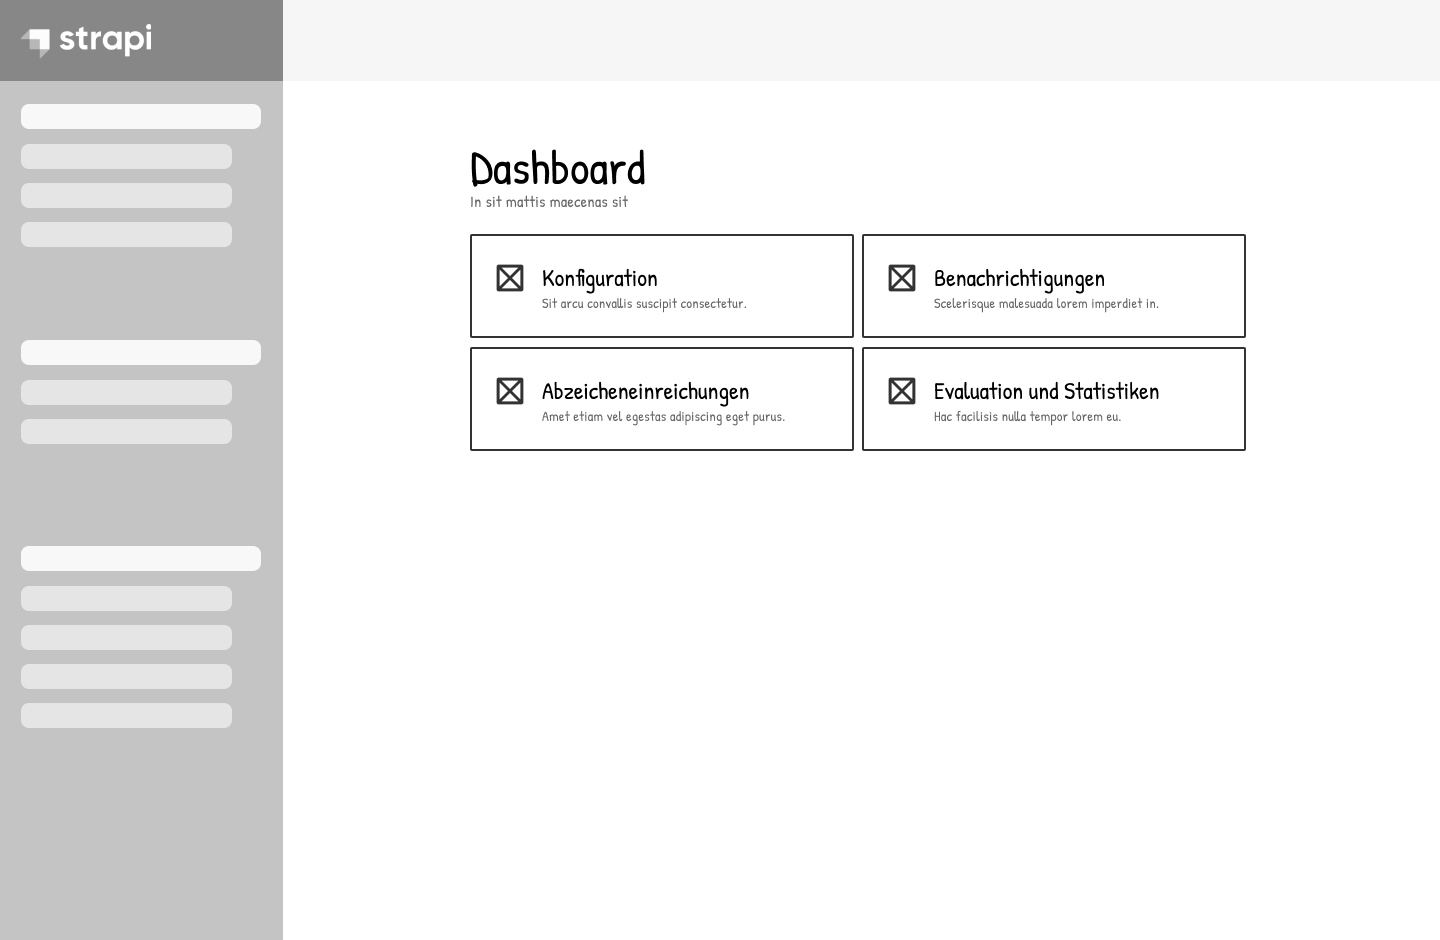
\includegraphics[width=\linewidth]{prototype/dashboard/dashboard.png}
    \caption{Startseite des Dashboards}
    \label{fig:prototype-dashboard-main}
\end{figure}

Die Funktionalitäten des Dashboards wurden in vier Kategorien gruppiert:
„Konfiguration“, „Benachrichtigungen“, „Abzeicheneinreichungen“ und „Evaluation
und Statistiken“. Auf der Startansicht des Dashboards werden diese vier
Kategorien in Form von Karten präsentiert (\autoref{fig:prototype-dashboard-main}). Jede Karte wird mit einem Icon
versehen, um die Kategorien visuell noch besser zu unterscheiden.

\begin{figure}[htpb]
    \centering
    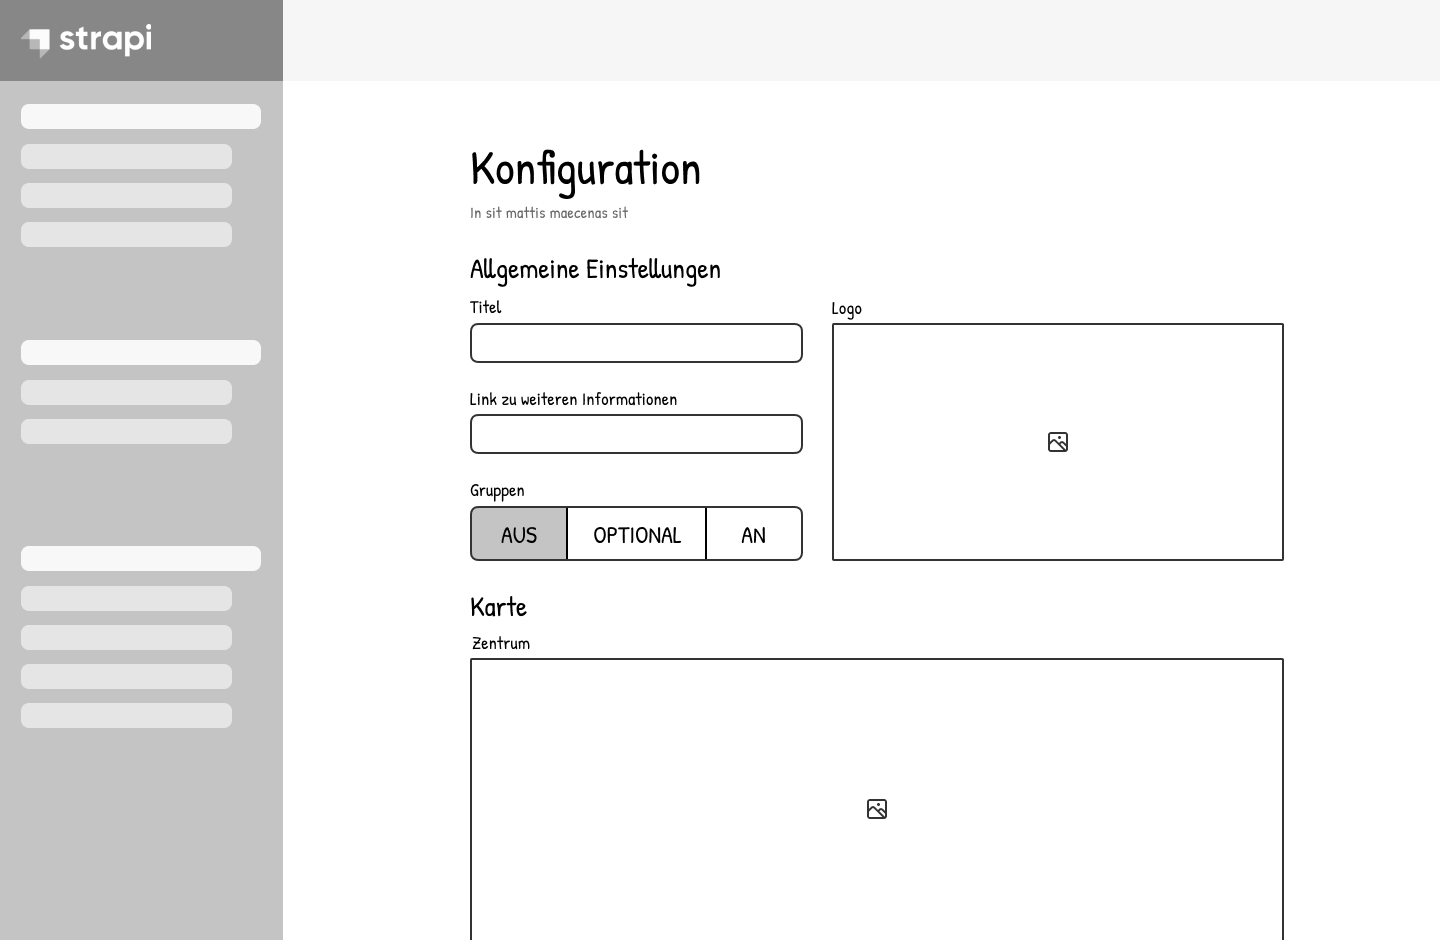
\includegraphics[width=\linewidth]{prototype/dashboard/configuration.png}
    \caption{Konfiguration der Rahmendaten der Veranstaltung}
    \label{fig:prototype-dashboard-config}
\end{figure}

Die Kategorie „Konfiguration“ beinhaltet die Einstellung der Rahmendaten der
Veranstaltung. Diese werden als Formular präsentiert (\autoref{fig:prototype-dashboard-config}). Die anzugebenden Daten sind hierbei
Titel, Logo, ein Link zu weiteren Informationen der Veranstaltung, die
Aktivierung der Gruppen-Funktion und das Zentrum der Karte. Zudem werden das
Impressum und die Datenschutzerklärung mithilfe von WYSIWYG-Editoren bearbeitet,
welche sich, nicht sichtbar, unter dem Zentrum der Karte befinden.

\begin{figure}[htb]
    \centering
    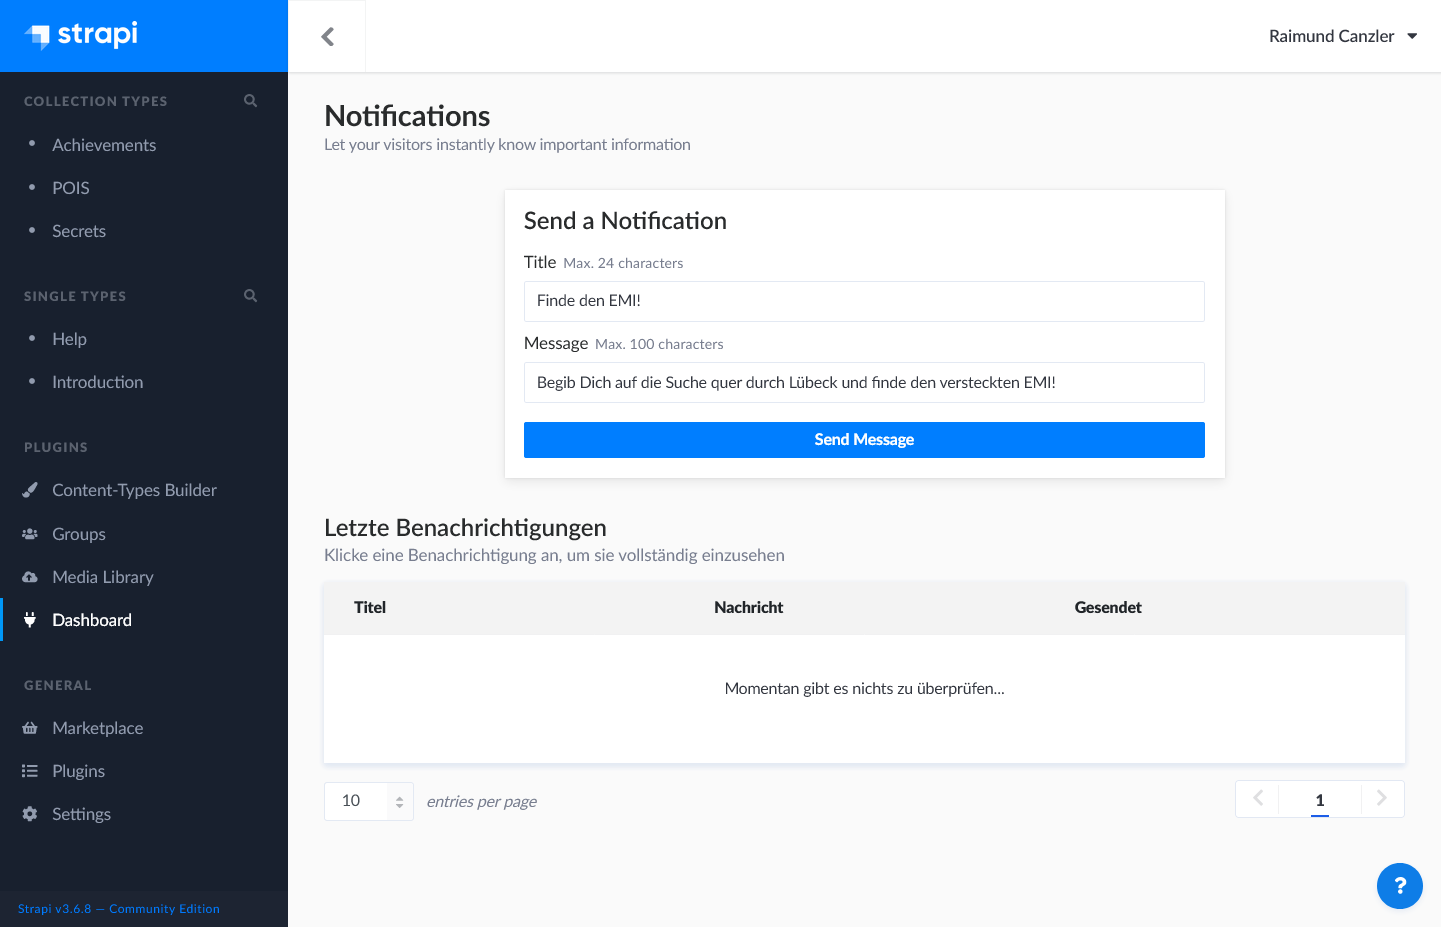
\includegraphics[width=\linewidth]{prototype/dashboard/notifications.png}
    \caption{Senden und Einsehen von Benachrichtigungen}
    \label{fig:prototype-dashboard-notifications}
\end{figure}

In der Kategorie „Benachrichtigungen“ können die Benachrichtigungen an
Teilnehmende gesendet werden. Hierzu kann das Formular im oberen Bereich des
Bildes genutzt werden (\autoref{fig:prototype-dashboard-notifications}).
Benachrichtigungen benötigen einen Titel und den Inhalt der Nachricht. Vor dem
Senden wird noch eine Bestätigung verlangt, um versehentlich abgeschickte
Nachrichten zu vermeiden (nicht visualisiert). Unterhalb des
Nachrichten-Formulars befindet sich eine Liste der bereits abgesendeten
Nachrichten. Die Liste gibt hierbei den Titel, die Nachricht und Datum sowie
Uhrzeit der jeweiligen Nachricht an. Da Nachrichten länger als die Breite der
Vorschau sein können, wird durch das Klicken auf eine Nachricht der Liste
zusätzlich ein Pop-up geöffnet, welches den vollen Inhalt der Nachricht anzeigt
(nicht visualisiert).

\begin{figure}[htpb]
    \centering
    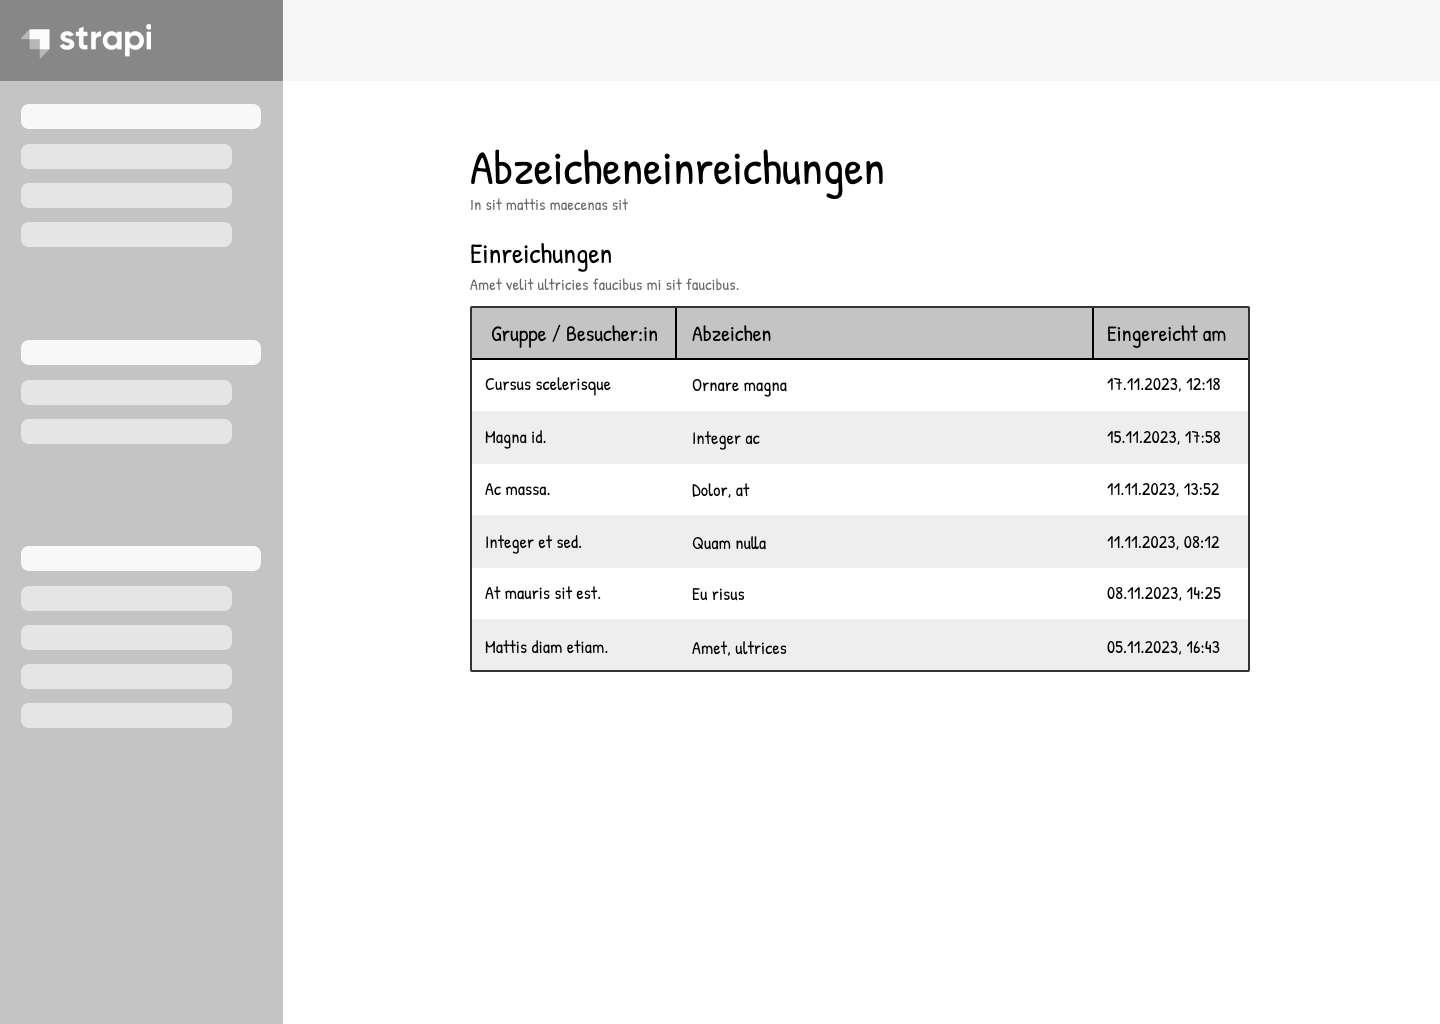
\includegraphics[width=\linewidth]{prototype/dashboard/submissions.png}
    \caption{Bewerten und Einsehen von Abzeicheneinreichungen}
    \label{fig:prototype-dashboard-submissions}
\end{figure}

\begin{figure}[htpb]
    \centering
    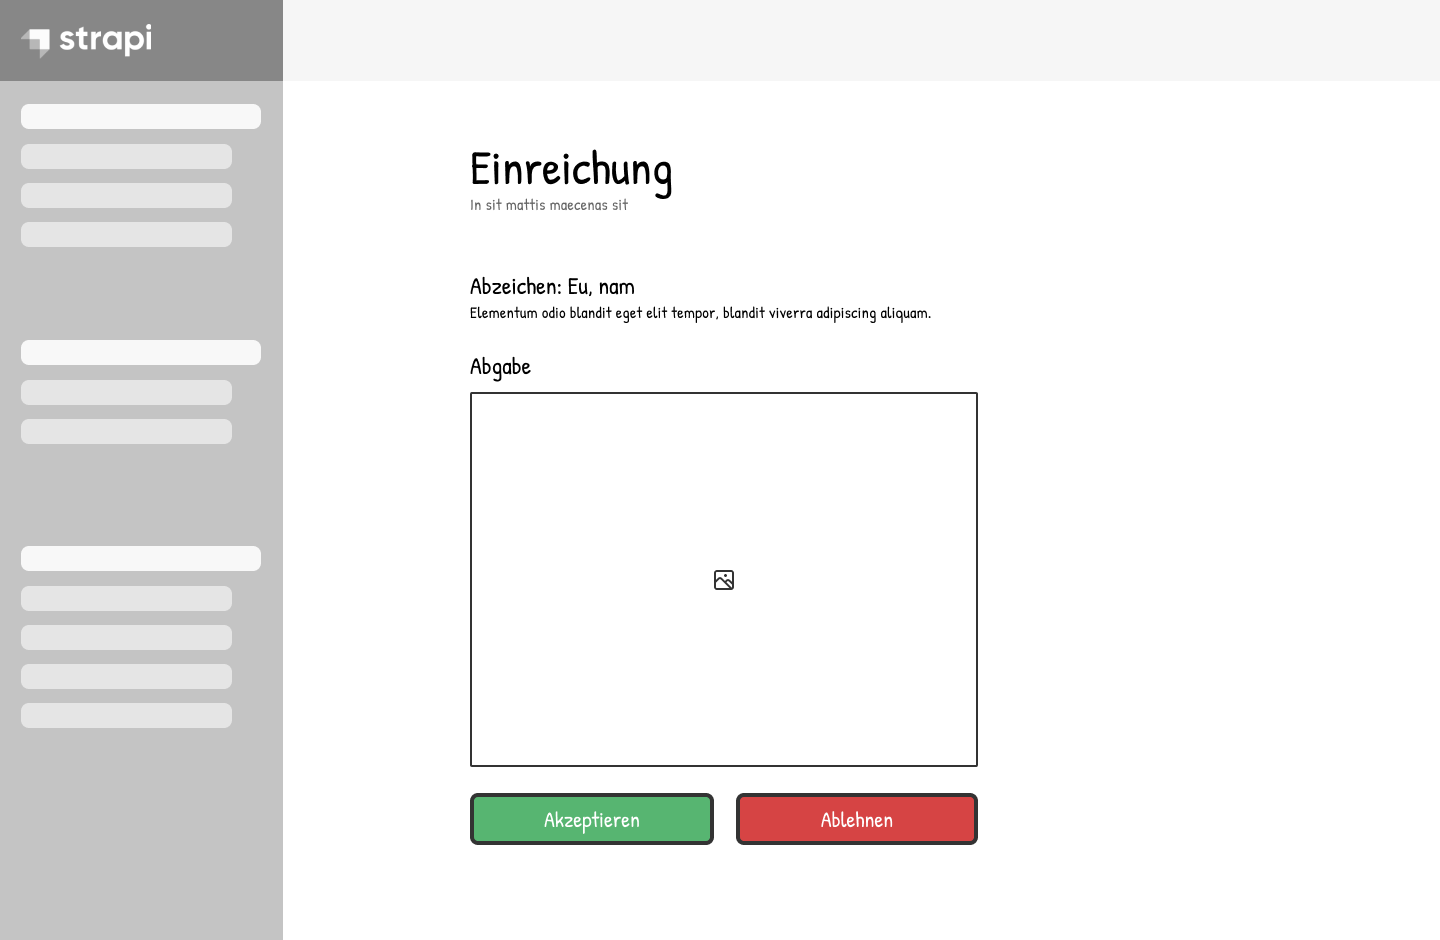
\includegraphics[width=\linewidth]{prototype/dashboard/submission.png}
    \caption{Bewerten einer Abzeicheneinreichung}
    \label{fig:prototype-dashboard-submission}
\end{figure}

Die Kategorie „Abzeicheneinreichungen“ bietet einen Weg die Einreichungen der
Teilnehmenden zu bewerten. Hierzu werden alle ausstehenden Bewertungen in Form
einer Liste, ähnlich zu den Benachrichtigungen, angezeigt (\autoref{fig:prototype-dashboard-submissions}). Die Liste zeigt den Namen der
Gruppe bzw. die ID der Besuchenden, das eingereichte Abzeichen und den
Zeitpunkt der Einreichung an. Durch das Anklicken einer Einreichung wird diese
geöffnet. Hier wird noch einmal das eingereichte Abzeichen und die
eigentliche Abgabe angezeigt (\autoref{fig:prototype-dashboard-submission}).
Die Abgabe kann je nach Text- oder Bildabzeichen, ein Text oder ein Bild sein.
Unter der Abgabe werden die beiden Bewertungsmöglichkeiten „Akzeptieren“ und
„Ablehnen“ angezeigt. Mit einem Klick auf eine der beiden Bewertungen wird die
Abgabe wieder geschlossen und aus der Liste entfernt.

\begin{figure}[htpb]
    \centering
    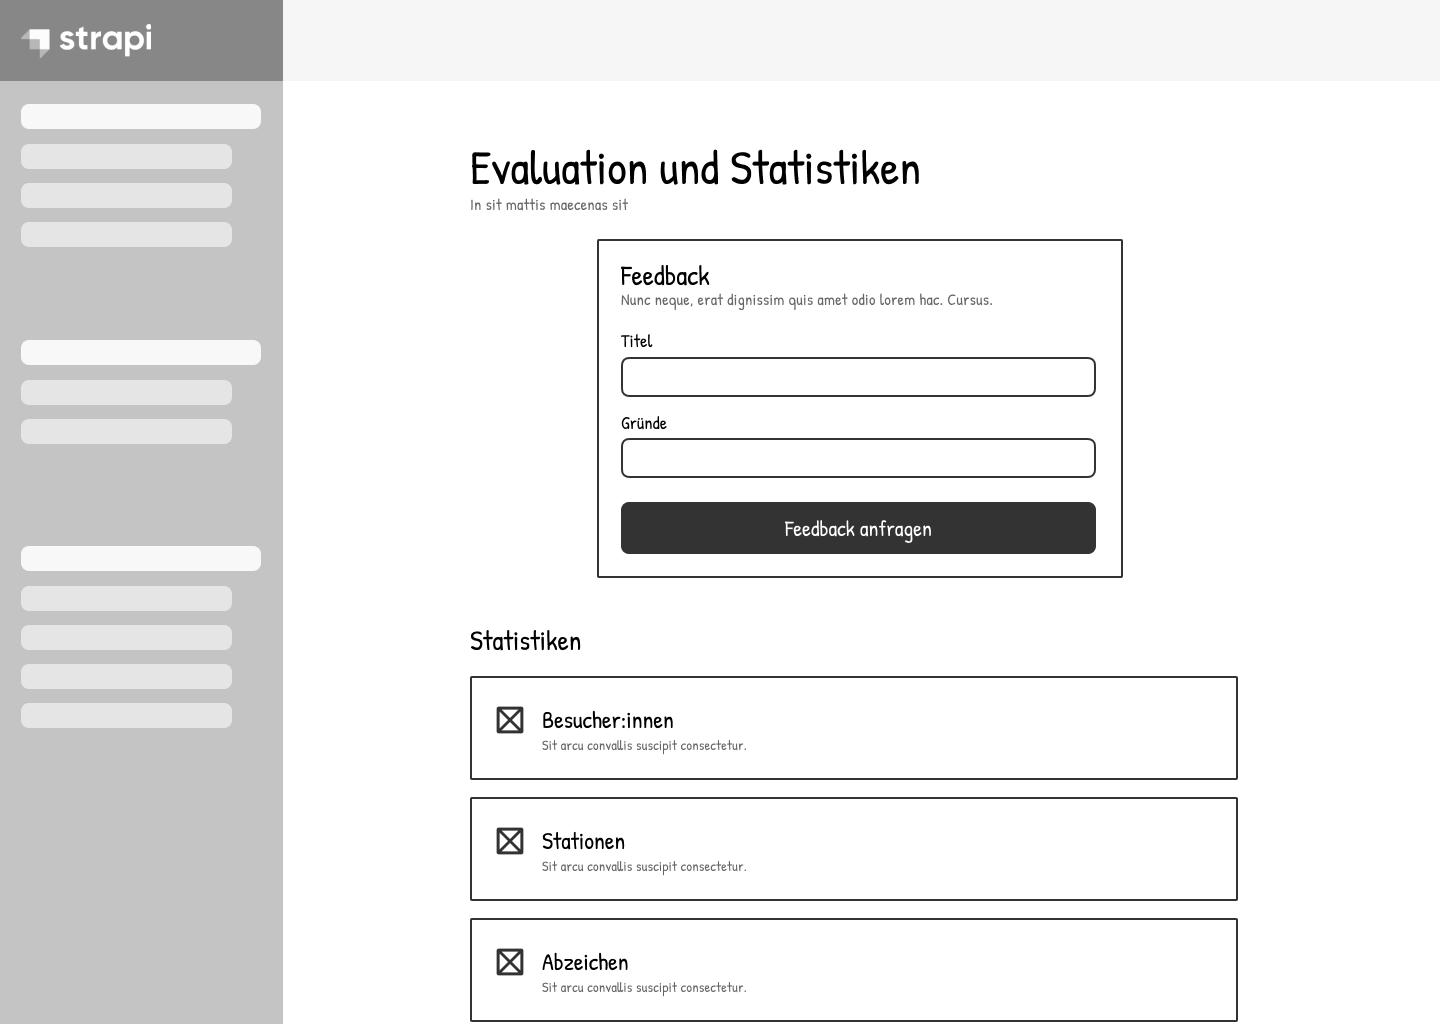
\includegraphics[width=\linewidth]{prototype/dashboard/evaluation_statistics.png}
    \caption{Feedback-Anfrage und Übersicht der Statistiken}
    \label{fig:prototype-dashboard-statistics}
\end{figure}

In der Kategorie „Evaluation und Statistiken“ finden sich zwei Funktionalitäten
wieder: Feedback-Anfragen und detaillierte Statistiken. Im oberen Bereich
befindet sich ein Formular zum Anfragen von Feedback (\autoref{fig:prototype-dashboard-statistics}). Dieses benötigt die Frage, zu der
Feedback gegeben werden soll, und optional Auswahlmöglichkeiten, welche als
Grund von negativem Feedback zur Auswahl stehen sollen. Auch dieses Formular
muss vor dem Senden bestätigt werden, um keine unbeabsichtigten Absendungen
zuzulassen. Unter dem Formular befinden sich Kacheln für die verschiedenen
Statistiken zu Besuchenden, Stationen, Abzeichen und Feedback-Anfragen. Durch
das Antippen einer Kachel wird zur entsprechenden Seite navigiert.

\begin{figure}[htpb]
    \centering
    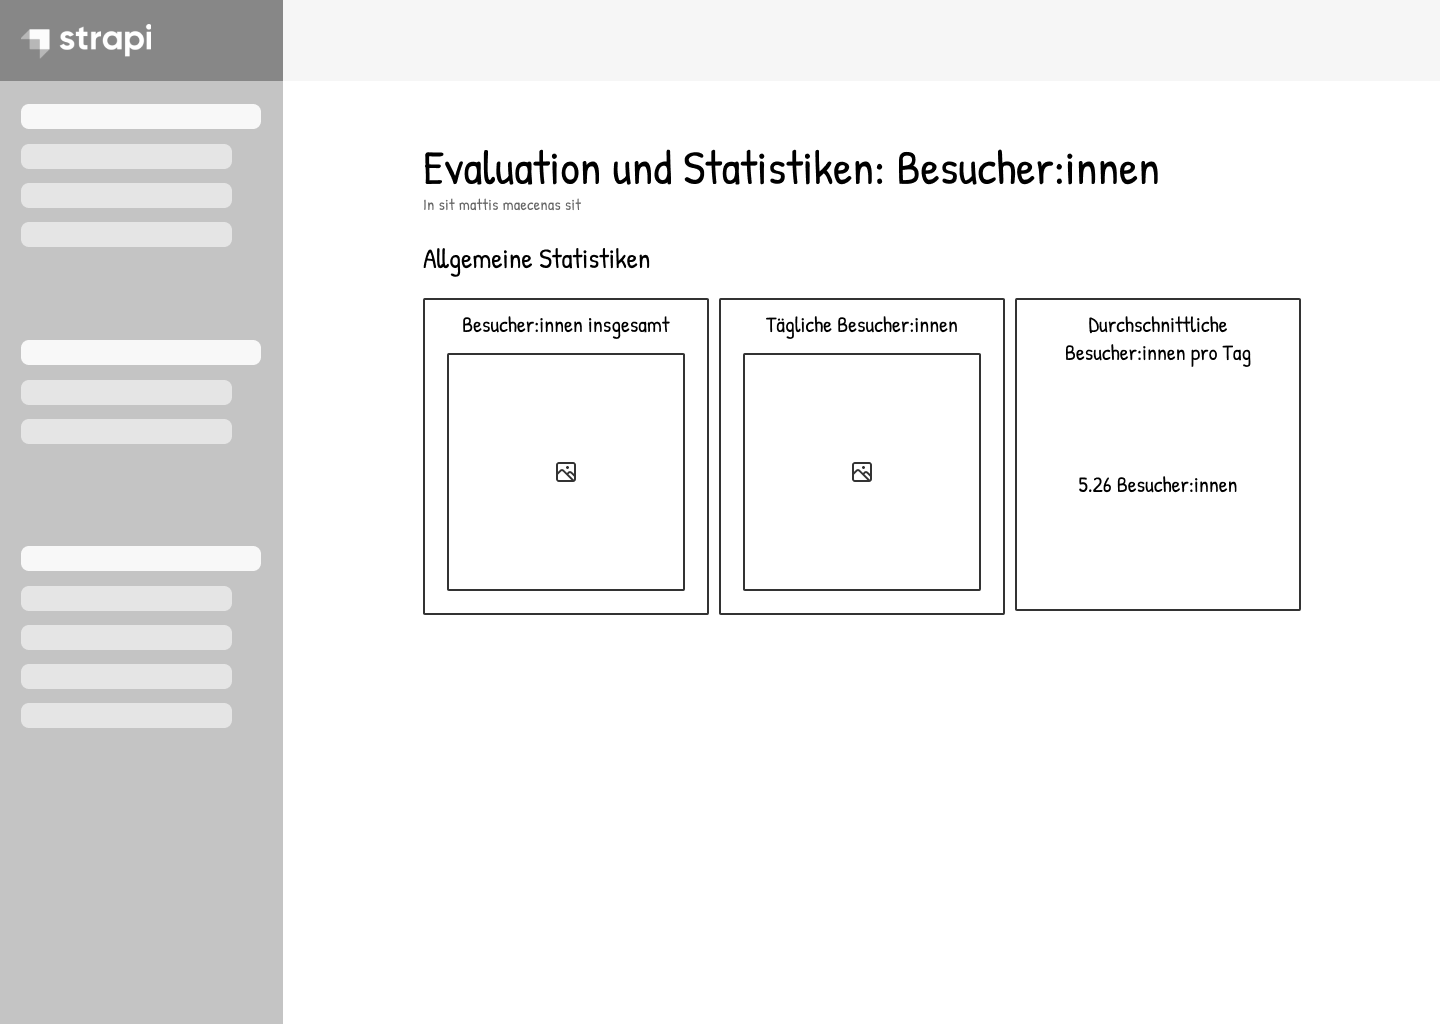
\includegraphics[width=\linewidth]{prototype/dashboard/statistics_visitor.png}
    \caption{Statistiken zu Besuchenden}
    \label{fig:prototype-dashboard-statistics-visitors}
\end{figure}

Auf der Seite der Besuchenden können drei verschiedene Statistiken eingesehen
werden: die kumulative Gesamtanzahl an Besuchenden, die neuen Besuchenden pro
Tag und die durchschnittliche Anzahl an neuen Besuchenden pro Tag (\autoref{fig:prototype-dashboard-statistics-visitors}). Die ersten
beiden Statistiken werden hierbei in Form eines Flächendiagramms angezeigt.

\begin{figure}[htpb]
    \centering
    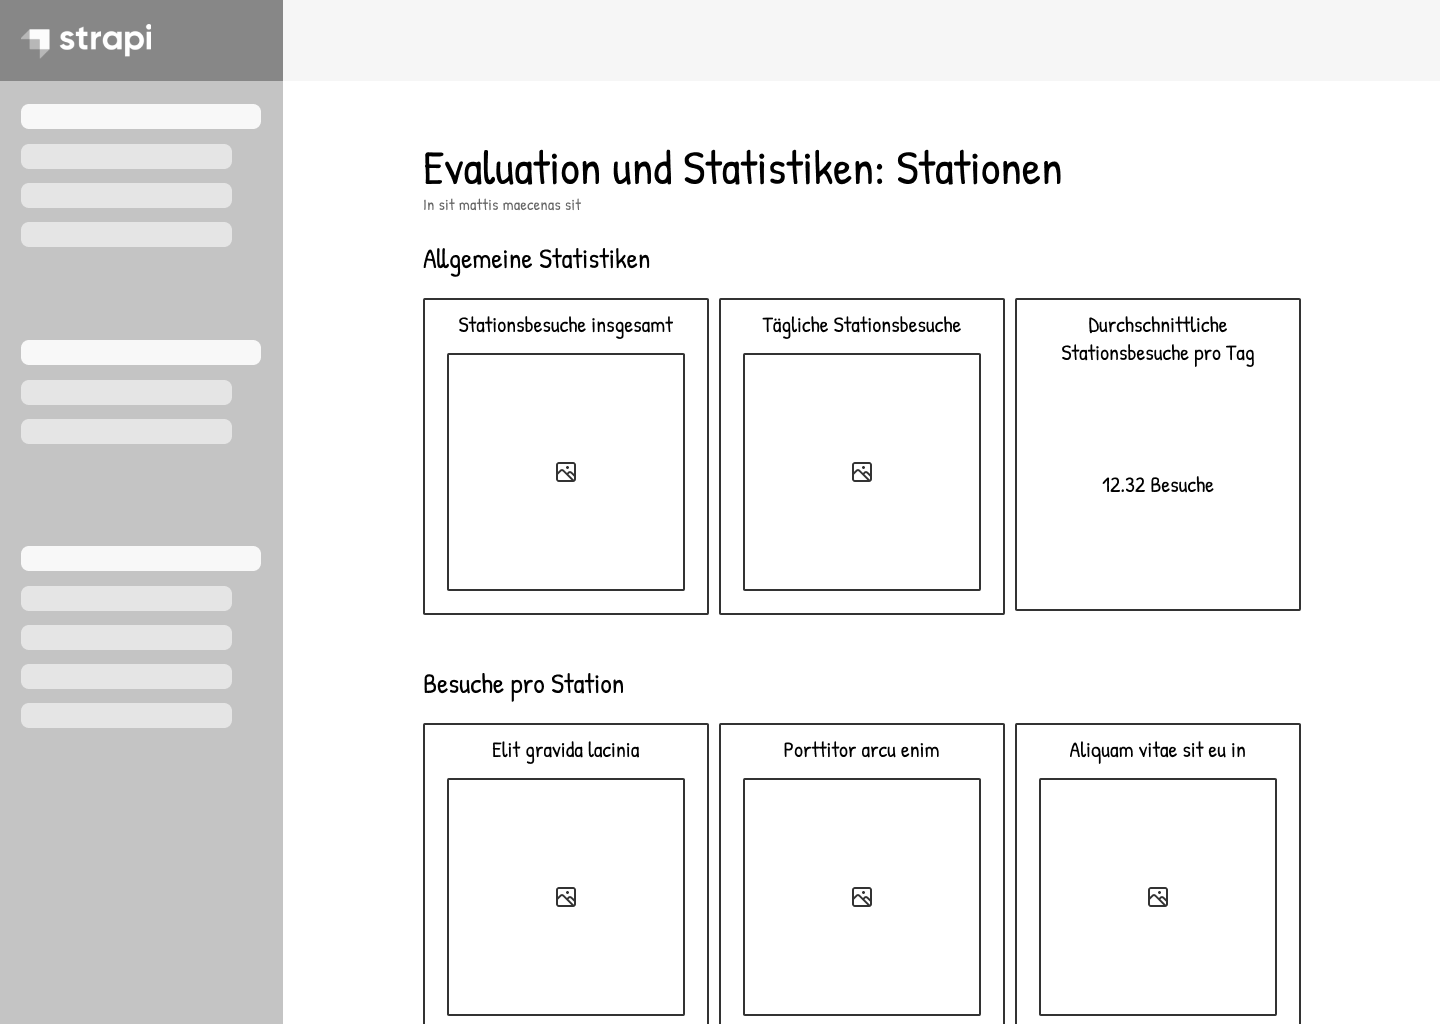
\includegraphics[width=\linewidth]{prototype/dashboard/statistics_stations.png}
    \caption{Statistiken zu Stationen}
    \label{fig:prototype-dashboard-statistics-stations}
\end{figure}

Auf der Seite der Stationen können anfangs ebenfalls drei verschiedene
Statistiken eingesehen werden: die kumulative Gesamtanzahl an Stationsbesuchen,
die neuen Stationsbesuche pro Tag und die durchschnittliche Anzahl an neuen
Stationsbesuchen pro Tag (\autoref{fig:prototype-dashboard-statistics-stations}). Die ersten beiden Statistiken werden auch hier in Form
eines Flächendiagramms angezeigt. Unter diesen allgemeinen Statistiken befinden
sich jedoch noch Flächendiagramme zu den einzelnen Stationen. Diese geben die
kumulative Gesamtanzahl an Stationsbesuchen der jeweiligen Station an. Hierbei
wird für jede Station ein Diagramm generiert. Analog wird es diese Seite auch
für die Abzeichen und Feedback-Anfragen geben.

\subsection{Teilnehmende}

Die Grundlage der Benutzeroberfläche der Teilnehmenden bildet die EMI-Award-App,
welcher im Rahmen des dazugehörigen Bachelorprojekts bereits evaluiert wurde. Es
wurden einige Anpassungen vorgenommen, um die Usability Heuristiken nach
\textcite{Nielsen1994} zu beachten (\anfref{Q40}). Diese werden im Folgenden
mit ihren IDs referenziert (vgl. \autoref{table:nielsen}).


\begin{table}[htpb]
    \def\arraystretch{1.25}
    \centering
    \caption{Die Zehn Usability Heuristiken \cite{Nielsen1994}}
    \label{table:nielsen}
    \begin{tabular}{ll}
        \uzlhline%
        \uzlemph{ID} & \uzlemph{Heuristik}                         \\
        \uzlhline%
        H1           & Sichtbarkeit des Systemstatus               \\
        H2           & Übereinstimmung von System und Wirklichkeit \\
        H4           & Beständigkeit und Standards                 \\
        H6           & Wiedererkennung statt Erinnerung            \\
        H7           & Flexibilität und Effizienz                  \\
        H8           & Ästhetisches und minimalistisches Design    \\
        H10          & Hilfe und Dokumentation                     \\
        \uzlhline
    \end{tabular}
\end{table}

Da auf dem Entwurf der EMI-Award-App aufgebaut wird, wurde direkt mit einem
High-Fidelity Prototypen begonnen. Dieser wurde ebenfalls mit Figma erstellt.
Das Design der EMI-Award-App ist spezifisch auf die dazugehörige Veranstaltung
abgestimmt. Um eine möglichst neutrale und anpassbare Darstellung zu ermöglichen
(\anfref{F130}), wurde das Design dementsprechend angepasst. Konkret wurde
bewusst auf Farben verzichtet und EMI-Award spezifische Grafiken entfernt oder
durch Platzhalter ersetzt. Allgemein wurde zudem die Schriftart und Schriftgröße
angepasst, um die Lesbarkeit nach dem \textcite{DBSV2022} zu gewährleisten. Als
Schriftart wurde \textit{Inter} gewählt, welche durch ihr hohes
Schriftgrößen-Mittellängen-Verhältnis (ca. 0.7, eigene Messung) besser lesbar
ist. Weiterhin wurde darauf geachtet, dass die Schriftgröße 16px nicht
unterschritten wird.

% Schriftart: Inter
% - Hohes Mittellängen-Schriftgrößen Verhältnis -> Sehr gut lesbar (DVSG)
%
% Schriftgröße: Laut DVSG Rechner mindestens 13px bei 30cm, 0.5 Visus, 0.7 MSV
% und 150 ppi

\begin{figure}[htpb]
    \begin{minipage}{.33\textwidth}
        \centering
        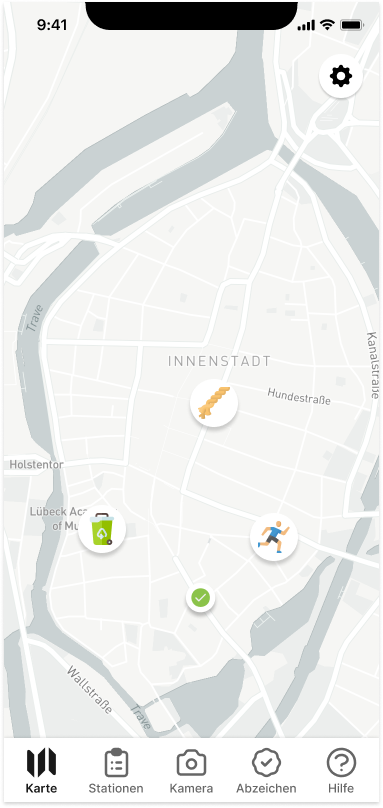
\includegraphics[width=.9\linewidth]{prototype/Karte.png}
    \end{minipage}%
    \begin{minipage}{.33\textwidth}
        \centering
        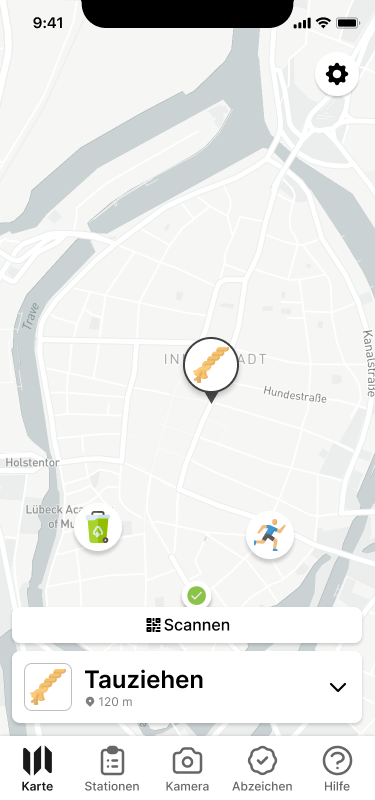
\includegraphics[width=.9\linewidth]{prototype/Karte-1.png}
    \end{minipage}
    \begin{minipage}{.33\textwidth}
        \centering
        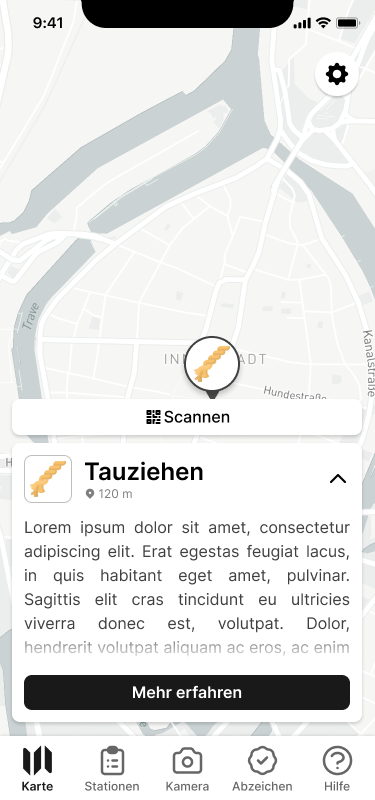
\includegraphics[width=.9\linewidth]{prototype/Karte-2.png}
    \end{minipage}
    \caption{Interaktive Karte mit Projektstandorten: nichts ausgewählt (links), ausgewählt (mittig), ausgewählt und aufgeklappt (rechts)}
    \label{fig:prototype-map}
\end{figure}

Aufgrund des variablen räumlichen Kontextes ist eine Verteilung der Stationen
über kilometergroße Räume möglich. Hierdurch ist die Distanz zu den
verschiedenen Stationen eine durchaus wichtige Information für Teilnehmende
(H2). Als Konsequenz wird die Distanz in verschiedenen relevanten Stellen des
User-Interfaces angezeigt. Eine dieser Stellen ist die interaktive Karte der
Stationen, insbesondere das Pop-up (\autoref{fig:prototype-map}, mittig). Jenes
wurde um die Distanz zur zugehörigen Station ergänzt. Des Weiteren wird die
Kurzbeschreibung standardmäßig eingeklappt, um Teilnehmende nicht mit zu vielen
Informationen zu konfrontieren (H7, H8). Zudem wird das Icon der Station nun
ebenfalls in das Pop-up eingebunden, da im Gegensatz zu den generischen Planeten
der EMI-Award-App die Icons der Stationen von Veranstaltenden selbst bestimmt
werden. Somit können die Icons mit den Stationen assoziiert werden, was die
Wiedererkennung im Rest der Benutzeroberfläche erleichtert (H6). Eine weitere
Ergänzung stellt ein „Jetzt Scannen“-Button dar, welcher direkt zur Kamera
navigiert, um die Navigation zu dieser zu erleichtern (H7) und gleichzeitig als
\textit{In-Context}-Hilfe dient (H6). Um den Fokus auf unbesuchte Stationen zu
lenken, werden besuchte Stationen zudem mit einem Haken als solche markiert und
kleiner dargestellt (\autoref{fig:prototype-map}, links). Zusätzlich können
besuchte Stationen auch komplett ausgeblendet werden. Beide Maßnahmen zielen
darauf ab, irrelevante Informationen auf der Benutzeroberfläche zu vermindern
oder zu vermeiden (H8). Hingegen wird die aktiv ausgewählte Station durch eine
Umrandung noch zusätzlich hervorgehoben. Insgesamt wird die Struktur und
Position des Pop-up angepasst, um sie populären Apps mit ähnlichen Funktionen
anzugleichen, da die Umgangsweise mit diesen bereits bekannt ist und somit
übertragen werden kann (H4).

% - Icons im Popup, da klein und durch Veranstalter bestimmbar statt generischer
%   Planet
% - Durch Distanz + Icon an Info dazu, sehr viele Informationen -> Ausblenden
%   von Sekundär Informationen (H8)

\begin{figure}[htpb]
    \centering
    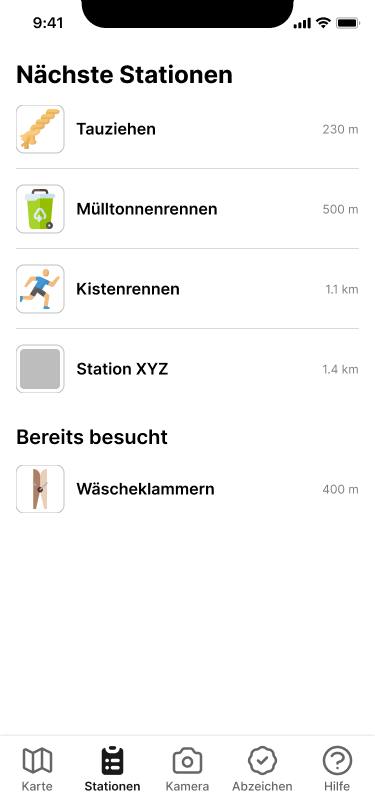
\includegraphics[width=.3\linewidth]{prototype/Stationen.png}
    \caption{Stationsauflistung}
    \label{fig:prototype-stations-list}
\end{figure}

Auch in der Stationsauflistung stellt die Distanz eine wichtige Information dar.
Somit wird für jeden Eintrag die Distanz angezeigt, wobei die Einträge
zusätzlich nach Distanz aufsteigend sortiert werden. Außerdem werden Stationen
nach „offen“ und „besucht“ gefiltert, wobei standardmäßig die Kategorie „offen“
angezeigt wird (\autoref{fig:prototype-stations-list}). Sowohl die Sortierung als auch die Filterung dienen dazu,
Teilnehmenden zuerst die relevantesten Informationen zu präsentieren (H8).
Konkret sind hiermit die nächstgelegenen unbesuchten Stationen gemeint. Des
Weiteren werden für die Einträge die jeweiligen Stationsicons verwendet. Diese
ersetzen die Bildvorschau der EMI-Award-App, da mediale Inhalte nicht mehr
zwingend benötigt werden, Icons hingegen schon.

\begin{figure}[htpb]
    \begin{minipage}{.5\textwidth}
        \centering
        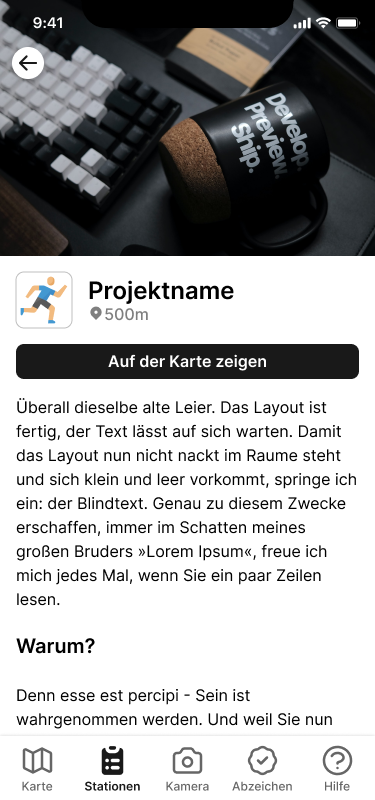
\includegraphics[width=.6\linewidth]{prototype/Stationen-1.png}
    \end{minipage}%
    \begin{minipage}{.5\textwidth}
        \centering
        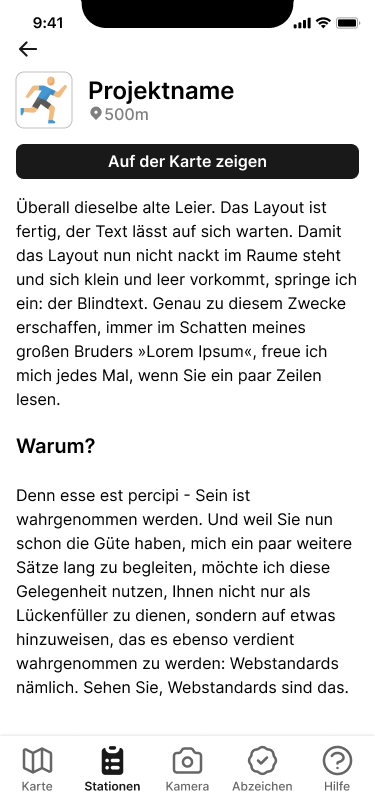
\includegraphics[width=.6\linewidth]{prototype/Stationen-2.png}
    \end{minipage}
    \caption{Stationsansicht: mit (links) und ohne (rechts) mediale Inhalte}
    \label{fig:prototype-stations-one}
\end{figure}

Die Stationsansicht wurde ebenfalls um die Distanz ergänzt und das
Wechseln zur Karte deutlich hervorgehoben. Da die Einbindung von medialen
Inhalten nicht zwingend erforderlich ist, wurde dies im Entwurf berücksichtigt
(vgl. \autoref{fig:prototype-stations-one}).

\begin{figure}[htpb]
    \begin{minipage}{.5\textwidth}
        \centering
        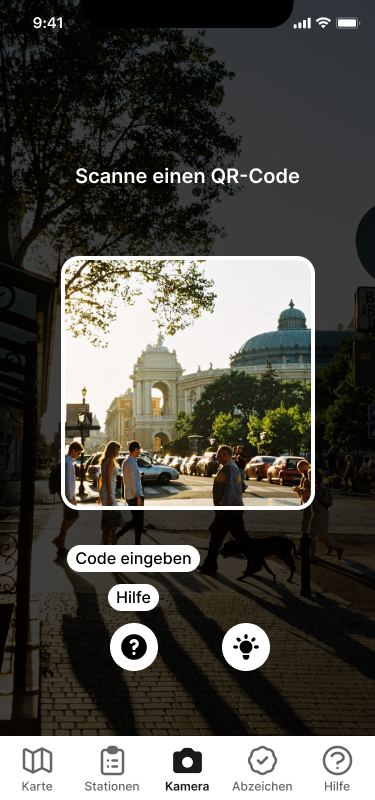
\includegraphics[width=.6\linewidth]{prototype/Kamera-1.png}
    \end{minipage}%
    \begin{minipage}{.5\textwidth}
        \centering
        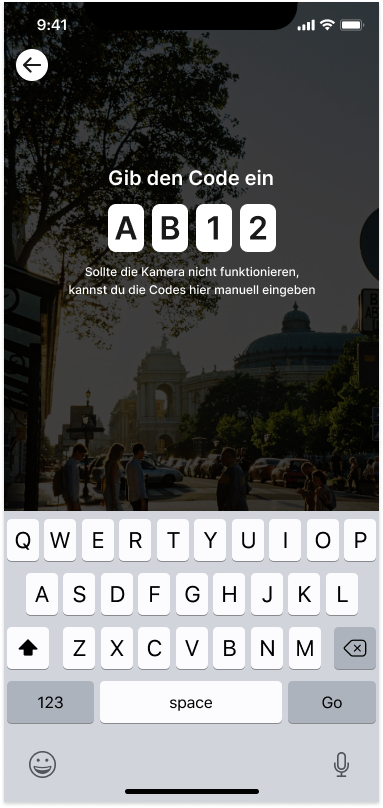
\includegraphics[width=.6\linewidth]{prototype/Kamera-2.png}
    \end{minipage}
    \caption{Kameraansicht: QR-Scanner (links) und manuelle Eingabe (rechts)}
    \label{fig:prototype-camera}
\end{figure}

Um die Scanner-Funktion der Kameraansicht ersichtlicher zu gestalten, wurde das
Design an gängige QR-Scanner angepasst (H4). Hierzu wurde der Scannerbereich mit
einem weißen Rand versehen und der restliche Bereich abgedunkelt (\autoref{fig:prototype-camera}). Zudem wurden die Icons zur verbesserten
Sichtbarkeit zentraler positioniert und zusammengeführt. Die manuelle
Codeeingabe und Hilfe sind mit dem Antippen des Fragezeichen-Icons erreichbar,
während die Taschenlampe angezeigt wird, wenn das Gerät die Funktionalität
unterstützt. Da die Codeeingabe nur schwer durch ein eindeutiges Icon
darstellbar ist, wurde sich bewusst entschieden, die Funktionalität auszuschreiben.

\begin{figure}[htpb]
    \begin{minipage}{.5\textwidth}
        \centering
        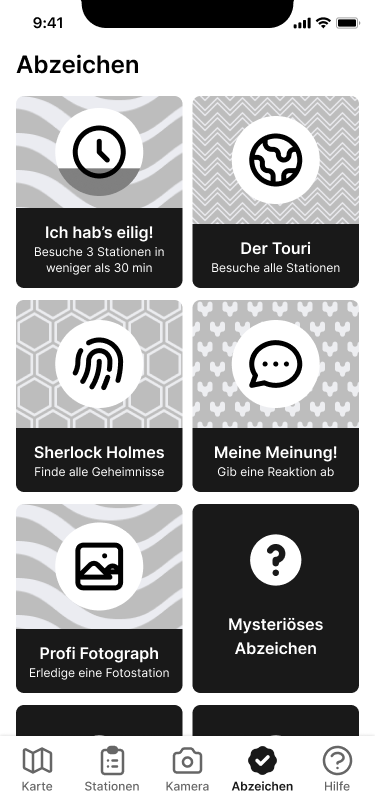
\includegraphics[width=.6\linewidth]{prototype/Abzeichen.png}
    \end{minipage}%
    \begin{minipage}{.5\textwidth}
        \centering
        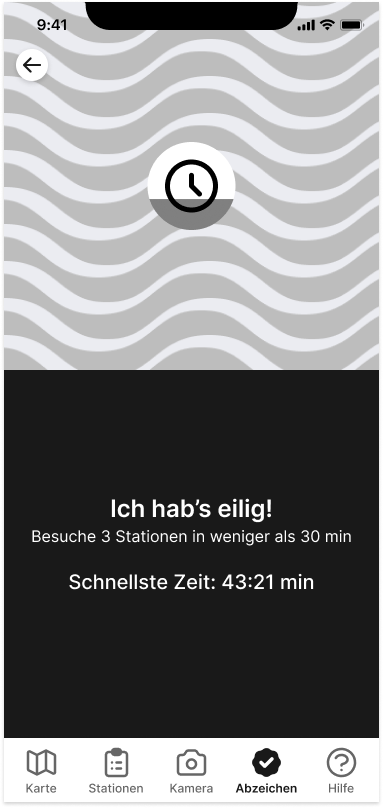
\includegraphics[width=.6\linewidth]{prototype/Abzeichen-1.png}
    \end{minipage}
    \caption{Abzeichen: Übersicht (links) und einzelne Ansicht (rechts)}
    \label{fig:prototype-achievement}
\end{figure}

Die einzelnen Abzeichen der Abzeichenansicht unterscheiden sich in der
EMI-Award-App lediglich durch ihre Farbe. Um Veranstaltenden möglichst viele
Freiheiten in der Anpassung zu geben, kann für jedes Abzeichen ein Icon
festgelegt werden. Dies ersetzt die festen Icons der EMI-Award-App. Zusätzlich
wird jedes Abzeichen mit einem zufälligen Muster hinterlegt (\autoref{fig:prototype-achievement}, links), um den Wiedererkennungswert und die
Differenzierbarkeit zu steigern. Außerdem erleichtert dies später die farbliche
Anpassung an die Veranstaltung (\anfref{F130}). Zudem wurde eine Einzelansicht
für Abzeichen hinzugefügt. Diese wird für die Text- und Bildabzeichen (Ft-T-8)
zum Einreichen benötigt und gibt Platz für ausführlichere Erklärungen oder
weiteren Informationen zu Abzeichen (\autoref{fig:prototype-achievement},
rechts).

\begin{figure}[htpb]
    \begin{minipage}{.5\textwidth}
        \centering
        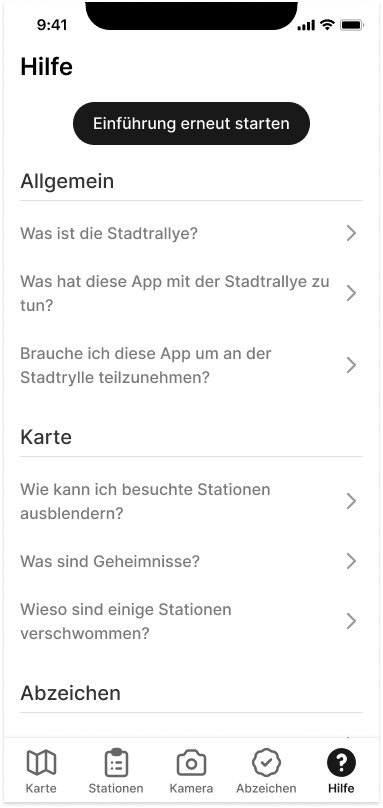
\includegraphics[width=.6\linewidth]{prototype/Hilfe.png}
    \end{minipage}%
    \begin{minipage}{.5\textwidth}
        \centering
        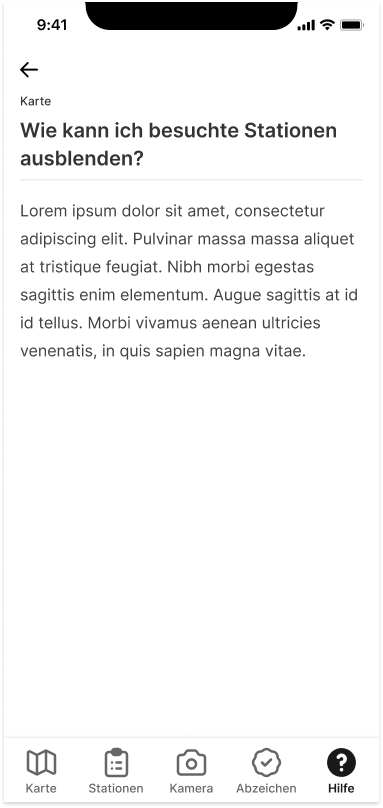
\includegraphics[width=.6\linewidth]{prototype/Hilfe-1.png}
    \end{minipage}
    \caption{Hilfe: Übersicht (links) und einzelne Ansicht (rechts)}
    \label{fig:prototype-help}
\end{figure}

Durch die in \autoref{sec:concept-func} beschriebenen Überarbeitung der
Hilfe-Funktion, muss die Benutzeroberfläche angepasst werden. Um die
Fragen übersichtlich anzuzeigen, werden sie nach den erstellten Kategorien
gruppiert präsentiert. Die Kategorien werden dabei durch die jeweilige
Überschrift abgegrenzt. Die Antwort zu den einzelnen Fragen wird wiederum in
einer Einzelansicht dargestellt. Zudem wird über einen Button im oberen Bereich
die Möglichkeit gegeben, die Einführung in die Veranstaltung (Ft-T-6) erneut zu durchlaufen.

\begin{figure}[htpb]
    \begin{minipage}{.5\textwidth}
        \centering
        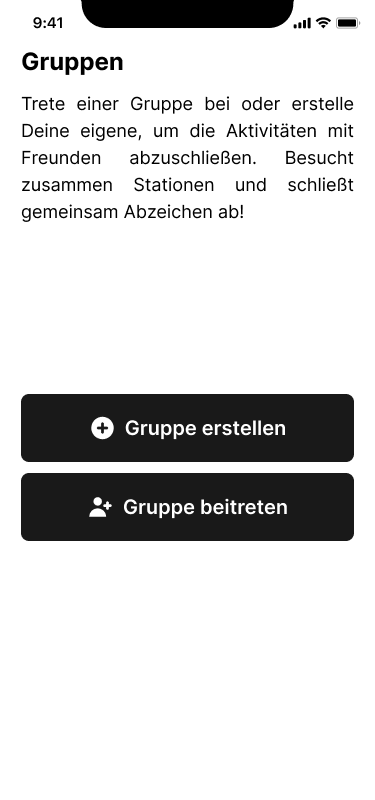
\includegraphics[width=.6\linewidth]{prototype/Gruppe.png}
    \end{minipage}%
    \begin{minipage}{.5\textwidth}
        \centering
        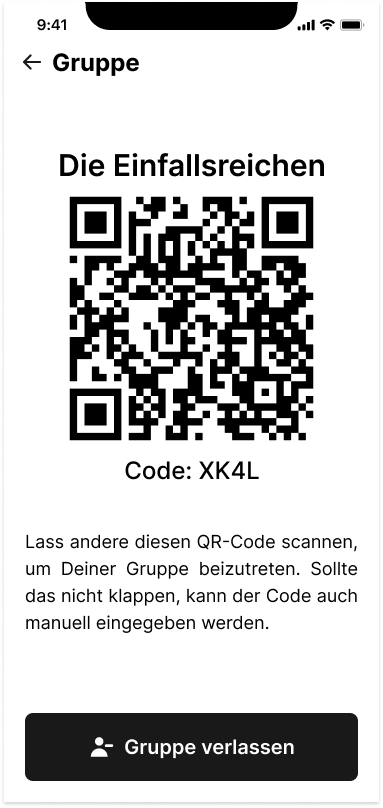
\includegraphics[width=.6\linewidth]{prototype/Gruppe-2.png}
    \end{minipage}
    \caption{Gruppen: Auswahl (links) und Mitgliederansicht (rechts)}
    \label{fig:prototype-groups-1}
\end{figure}

Zum Erstellen und Beitreten von Gruppen wurden zwei große Buttons verwendet,
welche ein passendes Icon nutzen, um die Funktion zu verdeutlichen (\autoref{fig:prototype-groups-1}, links). Sobald Teilnehmende Teil einer Gruppe
sind, werden Name, QR-Code und eine Anleitung angezeigt. Der Name dient der
Kontrolle, um Teilnehmenden zu zeigen, dass sie der richtigen Gruppe beigetreten
sind. Zum schnellen Beitreten kann der angezeigte QR-Code (\autoref{fig:prototype-groups-1}, rechts) verwendet werden. Sollte das Scannen
nicht funktionieren, kann über den darunter angezeigten Code manuell beigetreten
werden. Dies wird zudem in der Anleitung unter dem Code erklärt. Weiterhin haben
Teilnehmende am unteren Bildschirmrand die Möglichkeit die Gruppe zu verlassen.

\begin{figure}[htpb]
    \begin{minipage}{.5\textwidth}
        \centering
        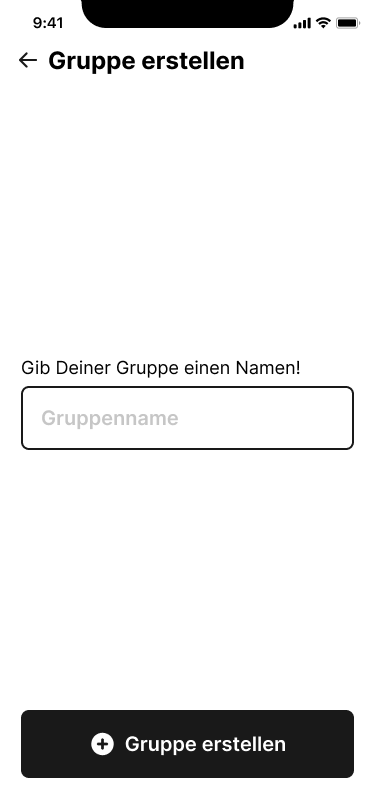
\includegraphics[width=.6\linewidth]{prototype/Gruppe-1.png}
    \end{minipage}%
    \begin{minipage}{.5\textwidth}
        \centering
        
\includegraphics[width=.6\linewidth]{prototype/Gruppe-3.png}
    \end{minipage}
    \caption{Gruppen: Erstellen (links) und Beitreten (rechts)}
    \label{fig:prototype-groups-2}
\end{figure}

Die Erstellungsansicht besteht lediglich aus einem Eingabefeld für den
Gruppennamen (vgl. \autoref{fig:prototype-groups-2}, links). Nachdem
Teilnehmende auf „Gruppe erstellen“ tippen, werden sie zur Mitgliederansicht aus
\autoref{fig:prototype-groups-1} weitergeleitet. Die Beitrittsansicht zeigt
hingegen einen QR-Code Scanner an, welche zum Scannen des Gruppen-QR-Codes
genutzt werden kann (\autoref{fig:prototype-groups-2}, rechts). Die manuelle
Eingabe des Gruppen-Codes kann über einen großen Button am unteren Rand des Bildschirms
erreicht werden.

\begin{figure}[htpb]
    \centering
    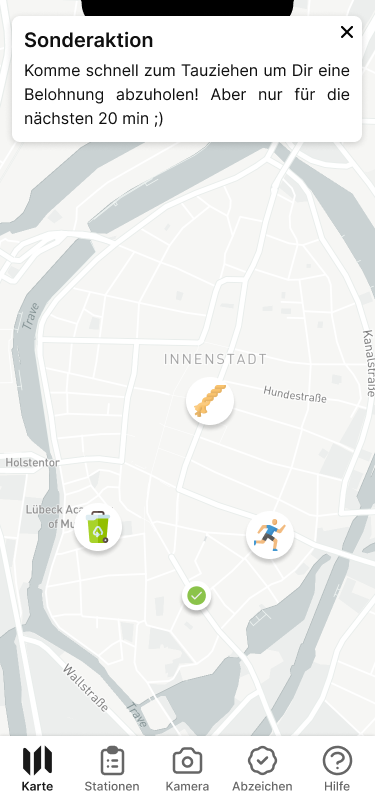
\includegraphics[width=.3\linewidth]{prototype/Notification.png}
    \caption{Benachrichtigung am oberen Bildschirmrand}
    \label{fig:prototype-notification}
\end{figure}

Falls Veranstaltende eine Benachrichtigung absenden, wird diese den
Teilnehmenden am oberen Bildschirmrand angezeigt (\autoref{fig:prototype-notification}). Die Benachrichtigung verschwindet dabei
nicht von allein und muss von den Teilnehmenden manuell geschlossen werden.
Somit wird sichergestellt, dass Teilnehmende die Benachrichtigung wahrnehmen.

\section{Systemarchitektur} \label{sec:system-architecture}

% Server & Datenbank - Strapi
% - Strapi Server
% - Strapi Oberfläche
% Web-App

Auf Grundlage der festgelegten Frameworks aus \autoref{sec:frameworks} wurde die
Systemarchitektur entworfen, welche eine Übersicht über die technische Umsetzung
des Systems gibt. Das System besteht im Wesentlichen aus zwei Komponenten: dem
Strapi \ac{CMS} und der Web-App (\anfref{R10}). Jedoch wird das Strapi \ac{CMS} zur Übersicht
in zwei weitere Teilkomponenten unterteilt: das Backend und die
Web-Oberfläche. Alle Komponenten und ihre Interaktionen werden im Folgenden
näher erläutert.

\subsection{Strapi: Backend}

Die Datenbank und API von Strapi bilden den Kern des Systems. Alle Stationen,
Stationsbesuche, Abzeichen, Benachrichtigungen und Rückmeldungen werden in der
Datenbank des Backends gespeichert und über die API für die anderen Komponenten
bereitgestellt. Die Logik für das Besuchen von Stationen und Abschließen von
Abzeichen wird im Backend untergebracht und mit der API für die Web-App
bereitgestellt.

\subsection{Strapi: Web-Oberfläche}

In der Web-Oberfläche von Strapi befindet sich das Dashboard für Veranstaltende.
Die darzustellenden Daten werden hierbei aus dem Backend abgerufen. Obwohl diese
Oberfläche ebenfalls von Strapi bereitgestellt wird, wie das eigentliche
Backend, ist die Funktion beider Komponenten klar voneinander getrennt. Die
Web-Oberfläche wird in React umgesetzt, da dies das von Strapi vorgegebene
Framework ist.

\subsection{Web-App}

Die Web-App stellt die Interaktionsfläche der Teilnehmenden dar. Auch die
Web-App greift auf das Backend zu, um darzustellende Daten abzurufen und
Aktionen, wie z. B. das Besuchen einer Station, durchzuführen. Die Web-App wird
separat von Strapi bereitgestellt und statisch gehostet. Das Generieren der
Web-App findet somit nur einmalig statt, im Gegensatz zum
Server-Rendering-Ansatz, bei welchem die Seite für jeden Aufruf neu generiert
werden muss.

\subsection{Interaktion der Komponenten}

Um die Interaktion der verschiedenen Komponenten übersichtlich zu
veranschaulichen, werden diese grafisch dargestellt (\autoref{fig:system-interaction}).

\begin{figure}[htpb]
    \renewcommand\baselinestretch{1}
    \centering
    \tikzset{
        arrow/.style={
                ->
            },
    }
    \tikz [thesis box shapes, baseline, anchor=base]{
        \coordinate (origin);

        \node [block] (WA) [above=of origin, xshift=4cm] {\textbf{Web-App}};
        \node [block] (SW) [above=of origin, xshift=-4cm] {\textbf{Strapi: Web-Oberfläche}};
        \node [block] (SB) [below=of origin] {\textbf{Strapi: Backend}};

        \draw[arrow] (WA.245) to (SB.50);
        \draw[arrow] (SB.30) to (WA.295);
        \draw[arrow] (SW.245) to (SB.150);
        \draw[arrow] (SB.130) to (SW.295);
    }
    \caption{Interaktion der Komponenten des Systems}
    \label{fig:system-interaction}
\end{figure}

%\section{Implikation für Implementierung}

% Gedanken zur technischen Umsetzung der EMI-App
%   - Vor-/Nachteile Web/Native
%   - Library Entscheidungen